\documentclass[12pt,a4paper]{article}
\usepackage[utf8]{inputenc}
\usepackage{geometry}
\usepackage{graphicx}
\usepackage{amsmath}
\usepackage{hyperref}
\usepackage{titlesec}
\usepackage{changepage}
\usepackage{caption}
\usepackage{float}
\usepackage{booktabs}
\usepackage{tabularx}
\usepackage[numbers]{natbib} % Menambahkan paket natbib untuk referensi
\usepackage{setspace} % Untuk mengatur spasi antar baris

% Page layout
\geometry{top=1in, bottom=1in, left=1in, right=1in}

% Modify section and subsection font size to normal
\titleformat{\section}[hang]{\normalsize\bfseries}{\thesection}{1em}{}
\titleformat{\subsection}[hang]{\normalsize\bfseries}{\thesubsection}{1em}{}

% Hanging indent for references
\setlength{\bibsep}{1em} % Mengatur jarak antar entri referensi
\setlength{\bibhang}{2em} % Mengatur indentasi menggantung untuk referensi

\begin{document}

% Title
\begin{titlepage}
    \centering
    {\Large\textbf{Deep Learning Course \\ Final Project Report}\par} % Judul
    \vspace{2cm} % Jarak antara judul dan logo
    
\includegraphics[width=0.5\linewidth]{Images/Logo-Resmi-Unhas-2.png}\par % Logo
    \vspace{2cm} % Jarak antara logo dan nama
    {\large
    Al Qadri (H071221052)\\ 
    Mifthahul Hoiri Bachruddin Basir (H071221072)\\ 
    Evan Pandu Nata (H071221057)\par}
    \vspace{1cm} % Jarak antara nama dan tanggal
     % Informasi universitas dan tanggal
    \textbf{Universitas Hasanuddin}\\
    \textbf{Makassar, Indonesia}\\[0.5cm]
    {\large\today\par} % Tanggal
\end{titlepage}

\normalsize  % Set the text size to normal for the entire document
\tableofcontents
\newpage

% 1. Introduction
\section{INTRODUCTION}
\subsection{Latar Belakang dan Konteks Proyek}
\begin{adjustwidth}{3em}{0pt} 
\hspace{0.5cm} Semaphore adalah salah satu metode komunikasi visual menggunakan bendera, yang secara historis digunakan dalam kondisi tertentu, seperti militer dan kelautan, ketika komunikasi verbal atau elektronik tidak memungkinkan. Setiap gerakan bendera melambangkan huruf dalam alfabet, sehingga membentuk pesan yang dapat dipahami. Namun, dengan berkurangnya penggunaan metode ini di era digital, kemampuan mengenali gerakan semaphore mulai memudar. Di sisi lain, pengembangan teknologi Artificial Intelligence (AI) dan Deep Learning memberikan peluang untuk menghidupkan kembali penerapan semaphore dalam konteks modern, seperti pengendalian lalu lintas, pelatihan keamanan, atau aplikasi edukasi.\end{adjustwidth}
\

\subsection{Masalah}
\begin{adjustwidth}{3em}{0pt} 
\hspace{0.5cm} Salah satu tantangan utama dalam pengembangan aplikasi berbasis AI untuk pengenalan gerakan semaphore adalah kurangnya dataset yang terorganisir dan mencakup seluruh alfabet semaphore (A-Z). Ketiadaan dataset ini menghambat pelatihan model deteksi objek yang andal. Selain itu, kebutuhan untuk mendeteksi gerakan semaphore secara real-time menjadi tantangan yang signifikan, terutama untuk aplikasi praktis seperti komunikasi darurat atau pelatihan. Tanpa dataset yang memadai, kemampuan model untuk mengenali gerakan semaphore dengan akurasi tinggi menjadi terbatas, sehingga mengurangi efektivitas teknologi ini di berbagai sektor. \end{adjustwidth}

\subsection{Tujuan}
\begin{adjustwidth}{3em}{0pt} 
\hspace{0.5cm} Proyek ini bertujuan untuk mengembangkan dataset lengkap gerakan bendera semaphore yang mencakup seluruh huruf A hingga Z, sebagai langkah awal dalam mendukung teknologi deteksi berbasis kecerdasan buatan. Dengan menggunakan model YOLOv8x, sistem diharapkan mampu mendeteksi gerakan semaphore secara otomatis dengan akurasi tinggi. Teknologi ini berpotensi mendukung aplikasi modern seperti komunikasi darurat, pendidikan, dan pelatihan keamanan. Selain itu, proyek ini bertujuan meningkatkan kemampuan sistem AI untuk mengenali gerakan semaphore secara real-time, sehingga dapat digunakan dalam berbagai kondisi praktis. Inisiatif ini juga mendorong pengembangan inovasi di bidang deteksi gerakan untuk menciptakan solusi yang relevan dan berkelanjutan.
\end{adjustwidth}

% \noindent Example:
% \lipsum[1] % Replace this with your content.

% 2. Related Works
\section{RELATED WORKS}
\begin{adjustwidth}{3em}{0pt} 
\hspace{0.5cm} Pengenalan gerakan semaphore dengan pendekatan teknologi berbasis kecerdasan buatan (Artificial Intelligence/AI) telah menjadi fokus perhatian berbagai penelitian dalam beberapa tahun terakhir. Inovasi ini didorong oleh kebutuhan untuk menciptakan sistem yang mampu mengenali gerakan semaphore secara otomatis, baik untuk tujuan komunikasi, pengajaran, maupun navigasi. Pangestu et al. mengembangkan sistem deteksi Bahasa Isyarat Indonesia (BISINDO) menggunakan algoritma YOLOv8. Dalam penelitian tersebut, algoritma YOLOv8 menunjukkan keunggulan signifikan dibandingkan versi sebelumnya dalam mendeteksi gerakan secara cepat dan akurat, khususnya dalam lingkungan yang membutuhkan respons real-time. Penelitian ini menjadi bukti bahwa YOLOv8 mampu menangani tantangan deteksi objek kecil dan menangkap detail gerakan yang kompleks, sehingga cocok untuk aplikasi pengenalan gestur.

\hspace{0.5cm} Halim et al. juga menyumbangkan kontribusi penting dengan mengembangkan aplikasi berbasis YOLO untuk pengenalan bahasa isyarat secara real-time. Hasil penelitian mereka menunjukkan bahwa algoritma YOLO sangat efisien untuk mendeteksi gerakan tubuh, meskipun masih terdapat tantangan dalam menangani variasi gerakan dan latar belakang yang dinamis. Selain itu, Amri memanfaatkan algoritma Convolutional Neural Network (CNN) untuk menerjemahkan bahasa isyarat menjadi teks atau suara. Pendekatan berbasis CNN ini memerlukan dataset yang besar dan terdiversifikasi untuk meningkatkan akurasi model, terutama dalam menangani gestur yang kompleks atau jarang digunakan.

\hspace{0.5cm} Dalam domain pengenalan gerakan semaphore secara spesifik, Motty et al. mengembangkan sistem deteksi menggunakan TensorFlow dan OpenCV. Meskipun sistem ini cukup andal dalam lingkungan terkendali, performanya cenderung menurun dalam latar belakang yang kompleks atau di bawah kondisi pencahayaan yang bervariasi. Di sisi lain, Budimartono et al. mengeksplorasi penggunaan sensor IMU untuk mengklasifikasikan gerakan semaphore dengan pendekatan berbasis CNN. Metode ini memberikan hasil yang baik dalam kondisi tertentu, tetapi memerlukan perangkat keras tambahan, sehingga kurang praktis untuk aplikasi sehari-hari. Mereka juga mengeksplorasi metode berbasis logika Fuzzy Mamdani, yang meskipun menawarkan interpretasi berbasis aturan, menghadapi keterbatasan dalam hal akurasi ketika diaplikasikan pada dataset yang lebih besar dan beragam. Penelitian lain oleh Gündoğdu dan Kumlu menggunakan metode ekstraksi fitur berbasis clustering untuk pengenalan gerakan semaphore. Meskipun pendekatan ini memberikan keunggulan dalam memahami pola fitur gerakan, metode ini kurang ideal untuk aplikasi real-time karena keterbatasan efisiensi komputasi.

\hspace{0.5cm} Dalam penelitian ini, kami memanfaatkan keunggulan model YOLOv8x, versi terbaru yang menawarkan kecepatan deteksi tinggi dan akurasi superior. Kami mengembangkan dataset khusus yang mencakup gerakan semaphore huruf A hingga Z dengan variasi sudut, pencahayaan, dan latar belakang untuk memastikan kemampuan model dalam menggeneralisasi berbagai kondisi. Pendekatan ini bertujuan untuk menjawab kekurangan yang ditemukan dalam penelitian sebelumnya, terutama terkait generalisasi model dalam lingkungan dunia nyata. Dengan menggunakan model YOLOv8x, kami berharap dapat menciptakan sistem yang tidak hanya akurat tetapi juga efisien untuk diterapkan dalam berbagai konteks praktis, seperti pengajaran, komunikasi, hingga navigasi berbasis isyarat semaphore. Penelitian ini diharapkan menjadi langkah maju dalam pengembangan teknologi pengenalan gerakan semaphore yang lebih andal dan aplikatif.
\end{adjustwidth}

% 3. Dataset and Material
\section{DATASET MATERIAL}
\subsection{Dataset}

Dalam proyek ini, kami membuat \textit{dataset} khusus untuk deteksi gerakan semaphore huruf A hingga Z melalui beberapa langkah berikut:

\subsubsection{Sumber Dataset}
\begin{itemize}
    \item Foto Teman: Gambar gerakan semaphore diambil secara langsung dari teman-teman yang berperan sebagai model. Proses pengambilan foto dilakukan di berbagai lokasi dengan variasi pencahayaan untuk memastikan keragaman kondisi dalam dataset.
    \begin{figure}[h]
        \centering
        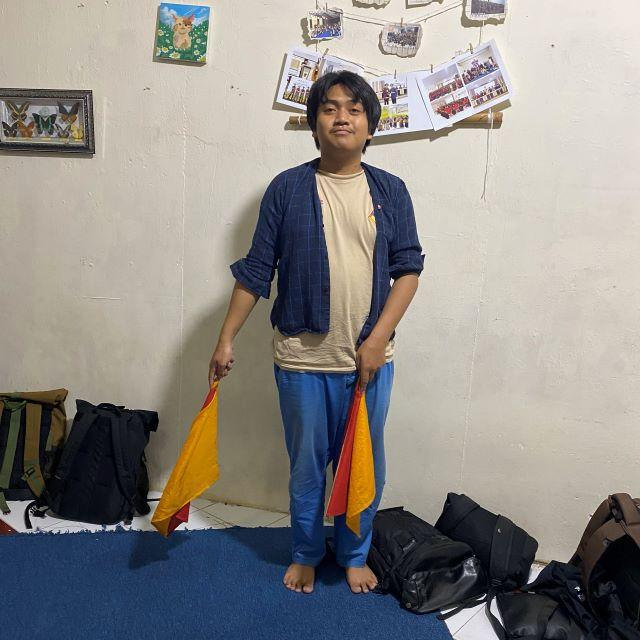
\includegraphics[width=0.6\linewidth]{Images/Gambar1.jpg}
        \caption*{Gambar 1. Pengambilan Gambar dengan Foto}
        \label{fig:enter-label}
    \end{figure}
    \item Video Teman: Rekaman video teman yang melakukan gerakan semaphore digunakan sebagai sumber tambahan. Video ini kemudian diproses menjadi frame individu untuk memperkaya variasi dataset. Dengan menggunakan video, kami dapat menangkap detail gerakan semaphore dalam berbagai sudut dan kecepatan.
    \begin{figure}[h]
        \centering
        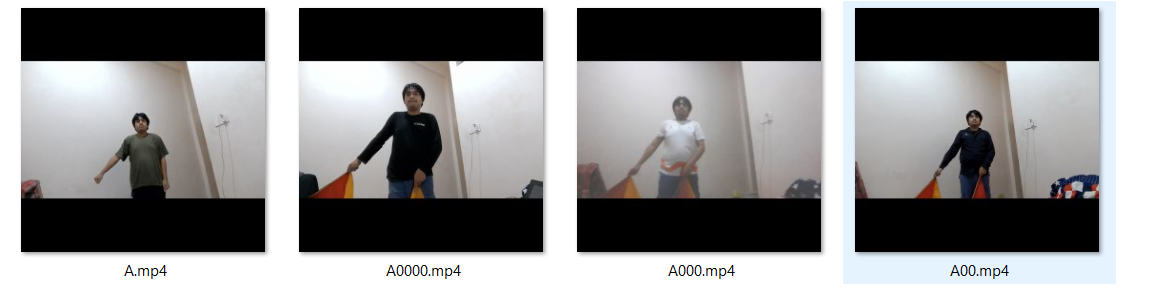
\includegraphics[width=0.9\linewidth]{Images/Gambar2.png}
        \caption*{Gambar 2. Pengambilan Gambar Dengan Video}
        \label{fig:enter-label}
    \end{figure}
\end{itemize}

\subsubsection{Prapemrosesan Dataset}
\begin{itemize}
    \item Pembersihan Data: Gambar atau frame yang tidak relevan atau berkualitas rendah (misalnya, buram, terlalu gelap, atau dengan posisi tangan yang tidak sesuai) dihapus untuk memastikan kualitas dataset yang optimal.
    \item Augmentasi Dataset: Seluruh gambar dan frame hasil ekstraksi diproses ulang agar memiliki ukuran square (1:1), yaitu 640 x 640 piksel, untuk memastikan keseragaman ukuran input ke model YOLOv8x. Augmentasi seperti rotasi, penyesuaian pencahayaan, dan pembalikan horizontal dilakukan untuk meningkatkan keragaman dataset.
    \item Anotasi (Labeling): Gambar yang telah dikumpulkan diunggah ke platform \textit{Roboflow} untuk anotasi manual. Setiap gambar diberi label berdasarkan huruf semaphore yang direpresentasikan, yaitu: 
    \begin{itemize}
        \item Huruf A-Z: Setiap gerakan semaphore dikategorikan sesuai huruf alfabet yang ditampilkan.
        \begin{figure}[h]
            \centering
            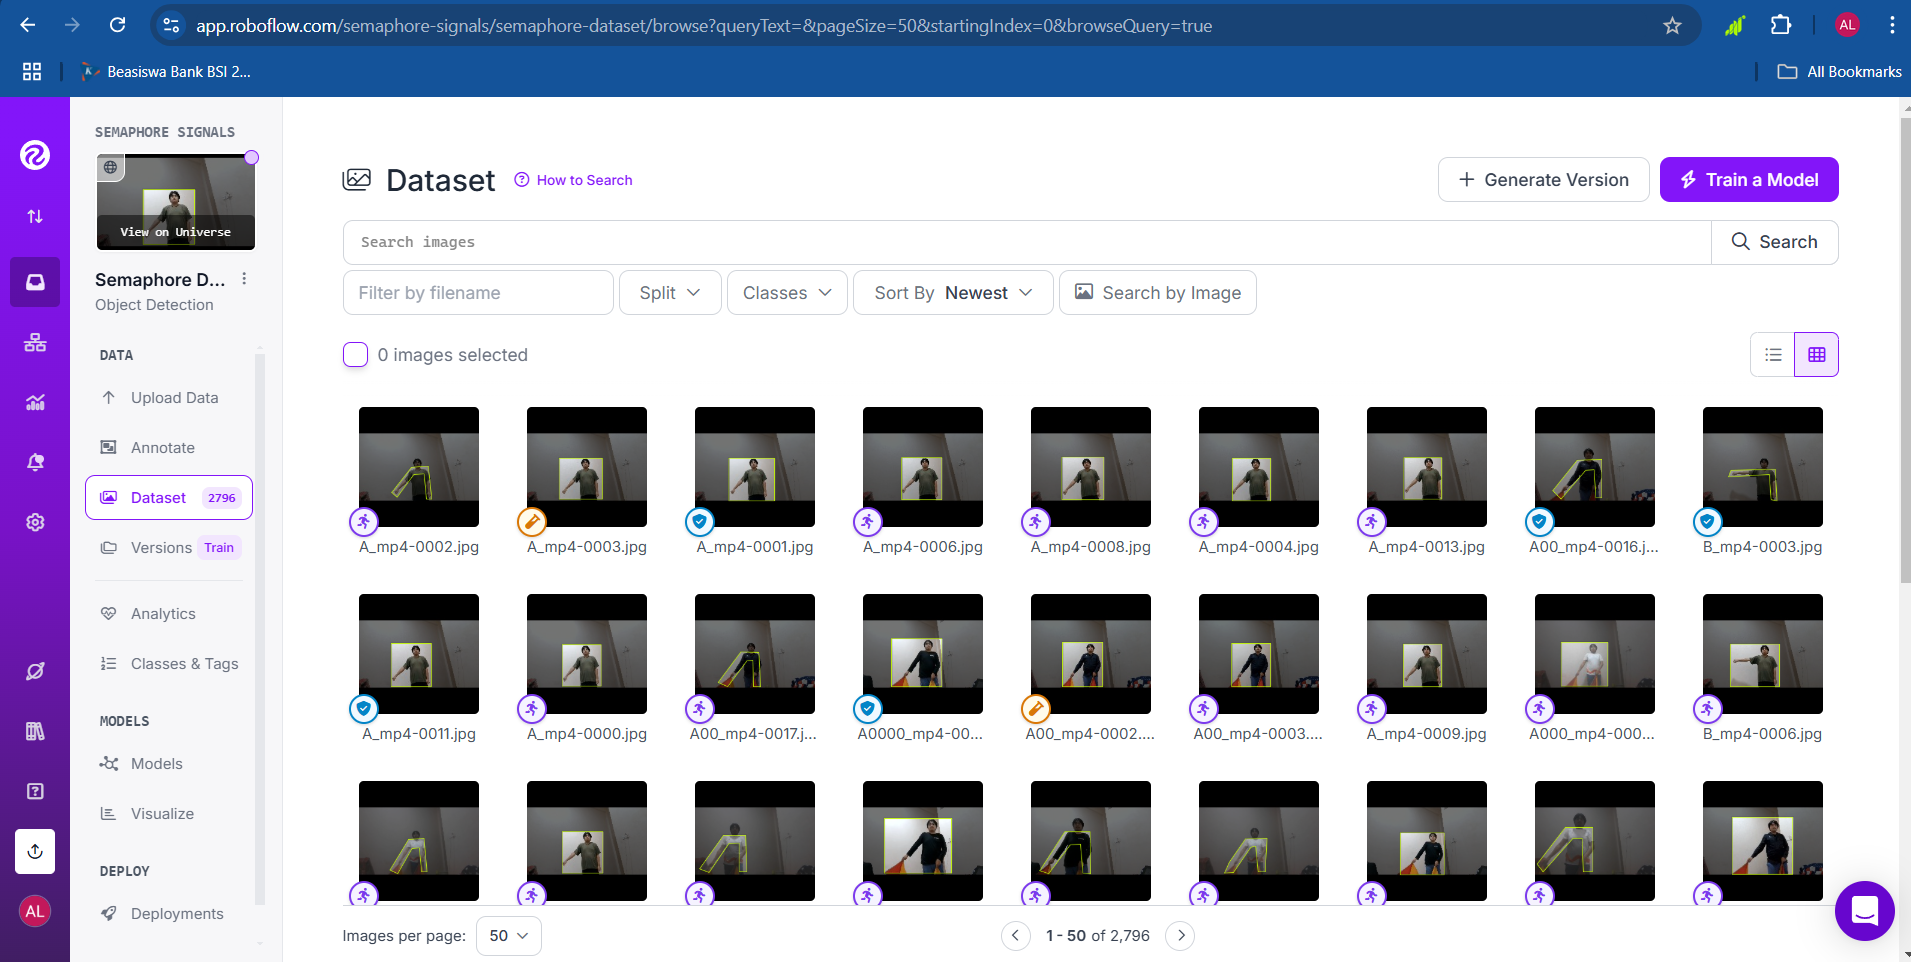
\includegraphics[width=0.8\linewidth]{Images/Gambar3.png}
            \caption*{Gambar 3. Anotasi di Roboflow}
            \label{fig:enter-label}
        \end{figure}
    \end{itemize}
\end{itemize}

\subsubsection{Karakteristik Dataset}
\begin{itemize}
    \item Jumlah Label:
    \begin{itemize}
        \item A: 131 label
        \item B: 113 label.
        \item C: 90 label.
        \item D: 91 label.
        \item E: 98 label.
        \item F: 89 label.
        \item G: 96 label
        \item H: 108 label.
        \item I: 106 label.
        \item J: 143 label
        \item K: 103 label.
        \item L: 101 label.
        \item M: 97 label
        \item N: 98 label.
        \item O: 116 label.
        \item P: 112 label
        \item Q: 111 label.
        \item R: 93 label.
        \item S: 109 label
        \item T: 105 label.
        \item U: 102 label.
        \item V: 115 label
        \item W: 129 label.
        \item X: 106 label.
        \item Y: 117 label.
        \item Z: 117 label.
        \begin{figure}[h]
            \centering
            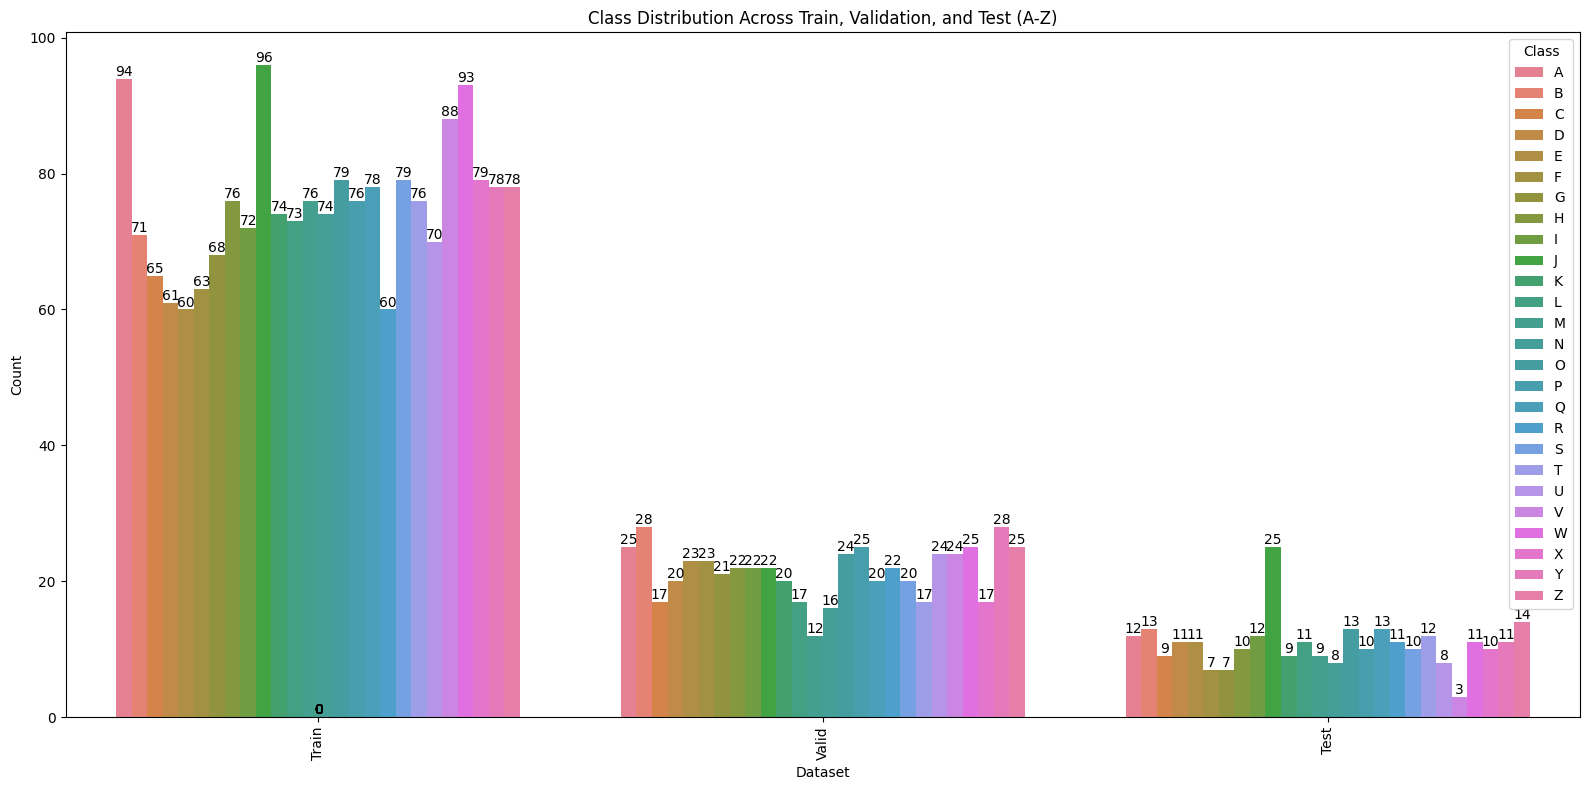
\includegraphics[width=0.9\linewidth]{Images/Gambar4.png}
            \caption*{Gambar 5. Distribusi Kelas Train, Validasi dan Test}
            \label{fig:enter-label}
        \end{figure}
    \end{itemize}
    \item Total Dataset: 2796 gambar setelah pembersihan data.
    \item Proporsi Data Berdasarkan Label:
    \begin{itemize}
        \item A: 4.69\%.
        \item B: 4.04\%.
        \item C: 3.22\%.
        \item D: 3.25\%.
        \item E: 3.51\%.
        \item F: 3.18\%.
        \item G: 3.43\%.
        \item H: 3.86\%.
        \item I: 3.79\%.
        \item J: 5.11\%.
        \item K: 3.68\%.
        \item L: 3.61\%.
        \item M: 3.47\%.
        \item N: 3.51\%.
        \item O: 4.15\%.
        \item P: 4.01\%.
        \item Q: 3.97\%.
        \item R: 3.33\%.
        \item S: 3.90\%.
        \item T: 3.76\%.
        \item U: 3.65\%.
        \item V: 4.11\%.
        \item W: 4.61\%.
        \item X: 3.79\%.
        \item Y: 4.18\%.
        \item Z: 4.18\%.
    \end{itemize}
    \item Format File: Semua gambar disimpan dalam format JPG/PNG dengan anotasi dalam format YOLO (bounding box).
\end{itemize}

\subsection{Material dan Alat}

\subsubsection{Alat dan Platform Anotasi}
\begin{itemize}
    \item Roboflow: Digunakan untuk mengunggah gambar gerakan semaphore, melakukan anotasi, dan mengelola dataset. Anotasi diekspor dalam format YOLO agar kompatibel dengan pelatihan model.
    \item Google Colab: Dimanfaatkan untuk pelatihan model dengan menggunakan GPU gratis untuk mempercepat proses komputasi.
\end{itemize}

\subsubsection{Pustaka dan Kerangka Kerja}
\begin{itemize}
    \item YOLOv8x: Model deteksi objek generasi terbaru yang digunakan untuk mendeteksi dan mengklasifikasikan gerakan semaphore dengan presisi tinggi.
    \item Numpy dan Pandas: : Digunakan untuk manipulasi data selama proses analisis \textit{dataset} seperti pemrosesan statistik dan transformasi data.
\end{itemize}

% 4. Result and Discussion
\section{RESULT AND DISCUSSION}
\subsection{Performance Metrics}
Tabel berikut menunjukkan performa model YOLOv5s dalam mendeteksi berbagai kategori gerakan bendera semaphore. Metrik yang digunakan untuk evaluasi adalah Precision, Recall, F1-Score, mAP50, dan mAP50-95.

\begin{figure}[h]
        \centering
        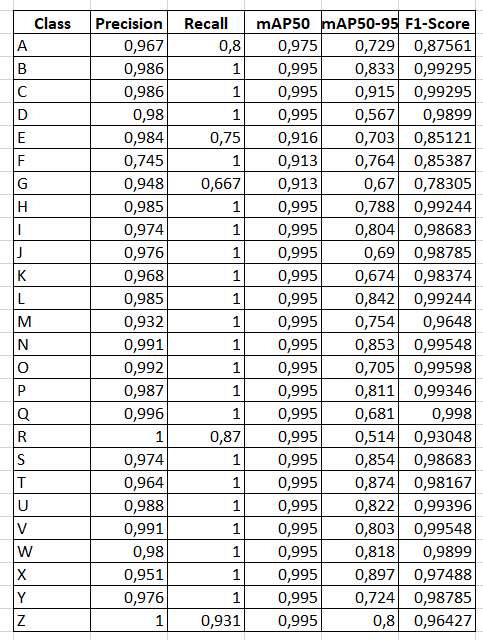
\includegraphics[width=0.6\linewidth]{Images/Gambar5Modelyolov5s.png}
        \caption*{Tabel 1. Metrik Evaluasi Model YOLOv5s}
        \label{fig:enter-label}
    \end{figure}
\begin{adjustwidth}{3em}{0pt} 
Dalam hal ini penggunaan YOLOv5s tidak digunakan karena Modelnya Masih dibawah daripada Model YOLOv8x. Tabel diatas menunjukkan performa model YOLOv5s dalam mendeteksi Gerakan Bendera Semaphore. Metrik yang digunakan adalah:

\begin{itemize}
    \item Precision: Mengukur akurasi model dalam memprediksi gerakan bendera, yaitu proporsi prediksi yang benar dari semua prediksi yang dihasilkan oleh model. Model ini menunjukkan presisi tertinggi pada kategori B, C, dan Z, dengan nilai 1, yang menunjukkan bahwa model tidak membuat kesalahan dalam memprediksi kategori tersebut.
    
    \item Recall: Mengukur kemampuan model dalam mendeteksi semua gerakan bendera yang ada, yaitu proporsi gerakan yang benar-benar terdeteksi dari seluruh gerakan yang ada. Beberapa kategori seperti B, C, H, dan I memiliki recall 1, yang berarti model berhasil mendeteksi semua gerakan dalam kategori ini.
    
    \item F1-Score: Merupakan rata-rata harmonik dari Precision dan Recall, yang memberikan gambaran umum tentang keseimbangan antara keduanya. F1-Score yang lebih tinggi menunjukkan performa yang lebih baik dalam mendeteksi gerakan dengan mempertimbangkan kedua metrik tersebut. Model ini menunjukkan F1-Score terbaik pada kategori Q, B, dan C dengan nilai sangat tinggi (0.998, 0.993, dan 0.993).
    
    \item mAP50: Mean Average Precision pada threshold IoU 0.5, yang menggambarkan akurasi model dalam mendeteksi objek pada level ketelitian tertentu. Kategori B dan C memiliki nilai mAP50 tertinggi (0.995), menandakan performa yang sangat baik dalam mendeteksi objek dengan ketelitian tinggi.

    \item mAP50-95: Mean Average Precision pada berbagai threshold IoU, memberikan gambaran performa model pada variasi toleransi deteksi. Beberapa kategori seperti C, S, dan T menunjukkan nilai mAP50-95 yang cukup tinggi, menunjukkan bahwa model dapat mendeteksi objek dengan toleransi yang lebih luas.
    
    \item Interpretasi: Model YOLOv5s menunjukkan kinerja yang baik pada sebagian besar kategori gerakan bendera semaphore, terutama untuk kategori seperti B, C, N, dan L, yang memiliki nilai mAP50, Precision, Recall, F1-Score, dan mAP50-95 yang sangat baik. Beberapa kategori seperti R, G, dan F menunjukkan hasil yang lebih rendah, terutama dalam hal Recall, F1-Score, dan mAP50-95, yang menunjukkan ada ruang untuk perbaikan dalam mendeteksi gerakan tersebut secara lebih akurat.
    
Secara keseluruhan, model YOLOv5s memberikan hasil yang sangat baik untuk deteksi gerakan bendera semaphore, meskipun beberapa kategori menunjukkan kebutuhan untuk perbaikan lebih lanjut guna mencapai akurasi deteksi yang lebih optimal. 
\end{itemize}
\end{adjustwidth}

Tabel berikut menunjukkan performa model YOLOv5s dalam mendeteksi berbagai kategori gerakan bendera semaphore. Metrik yang digunakan untuk evaluasi adalah Precision, Recall, F1-Score, mAP50, dan mAP50-95.

\begin{figure}[h]
        \centering
        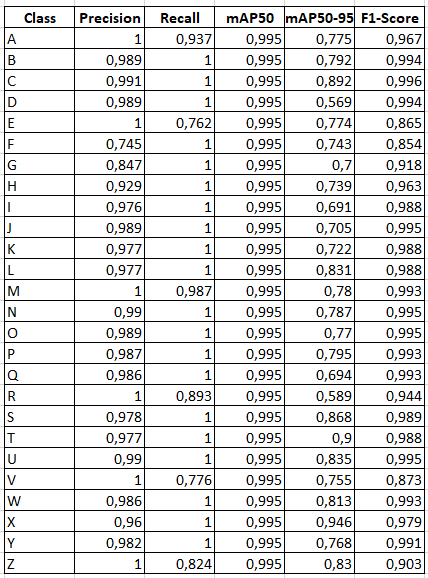
\includegraphics[width=0.6\linewidth]{Images/Gambar6Modelyolov8x.png}
        \caption*{Tabel 2. Metrik Evaluasi Model YOLOv5s}
        \label{fig:enter-label}
    \end{figure}
\begin{adjustwidth}{3em}{0pt} 

\begin{itemize}
    \item mAP50: Mengukur rata-rata presisi untuk semua kategori pada threshold IoU 0.5. Nilai ini menunjukkan akurasi model dalam menentukan posisi dan keberhasilan mendeteksi gerakan bendera semaphore. Pada tabel di atas, kategori B (gerakan bendera) memiliki nilai mAP50 tertinggi (0.995), yang menunjukkan performa model yang sangat baik dalam mendeteksi kategori tersebut. Meskipun beberapa kategori seperti G atau F memiliki nilai mAP50 sedikit lebih rendah, mereka tetap menunjukkan hasil yang cukup baik, dengan nilai masing-masing 0.972 dan 0.879, yang masih memadai dalam konteks deteksi objek.

    
    \item Precision: Mengukur akurasi prediksi model, yaitu proporsi prediksi gerakan bendera yang benar dari semua prediksi yang dihasilkan oleh model. Model memiliki presisi tertinggi pada kategori B dan C, dengan nilai 1, yang menandakan tidak ada kesalahan dalam prediksi untuk kategori ini. Kategori F memiliki presisi terendah (0.745), namun masih menunjukkan hasil yang cukup baik meskipun ada beberapa kesalahan prediksi pada kategori ini.

    
    \item Recall: Mengukur kemampuan model dalam mendeteksi gerakan yang benar, yaitu proporsi gerakan yang benar-benar terdeteksi dari seluruh gerakan yang ada. Recall tertinggi ditemukan pada kategori B, H, dan beberapa kategori lainnya, yang masing-masing memiliki recall 1, menunjukkan bahwa model dapat mendeteksi semua contoh pada kategori tersebut tanpa gagal.Kategori G memiliki recall lebih rendah (0.667), yang menunjukkan bahwa model belum sepenuhnya mampu mendeteksi semua gerakan dengan akurat, sehingga masih ada ruang untuk peningkatan.
    
    \item F1-Score: : Kombinasi antara precision dan recall yang memberikan keseimbangan antara keduanya. F1-Score tertinggi ada pada kategori C, B, dan P, yang memiliki nilai sangat mendekati 1, menandakan keseimbangan yang baik antara precision dan recall.Kategori F menunjukkan nilai F1-Score lebih rendah (0.853), namun tetap memadai untuk aplikasi ini, meskipun ada ruang untuk perbaikan lebih lanjut dalam hal keseimbangan antara precision dan recall.

    \item mAP50-95: Mean Average Precision pada beberapa threshold IoU, memberikan gambaran performa model pada variasi toleransi deteksi.
    
    \item Interpretasi: Model YOLOv8x menunjukkan performa yang sangat baik pada sebagian besar kategori gerakan bendera semaphore, terutama pada kategori yang memiliki nilai mAP50, Precision, Recall, dan F1-Score yang sangat tinggi seperti B, H, dan C. Kategori-kategori ini menunjukkan bahwa model mampu mendeteksi gerakan dengan akurat dan seimbang antara precision dan recall. Namun, untuk kategori G dan F, performa sedikit menurun. Misalnya, kategori G memiliki nilai recall yang lebih rendah (0.667), yang menunjukkan bahwa model belum sepenuhnya mampu mendeteksi semua gerakan dengan akurat. Begitu juga dengan kategori F, yang memiliki presisi lebih rendah dan F1-Score yang sedikit lebih rendah dibandingkan kategori lainnya.
      
Secara keseluruhan, model ini menunjukkan kinerja yang sangat baik dalam mendeteksi gerakan bendera semaphore, namun ada beberapa kategori yang memerlukan perbaikan lebih lanjut untuk mencapai hasil yang lebih optimal. 
\end{itemize}
\end{adjustwidth}

\begin{figure}[h]
    \centering
    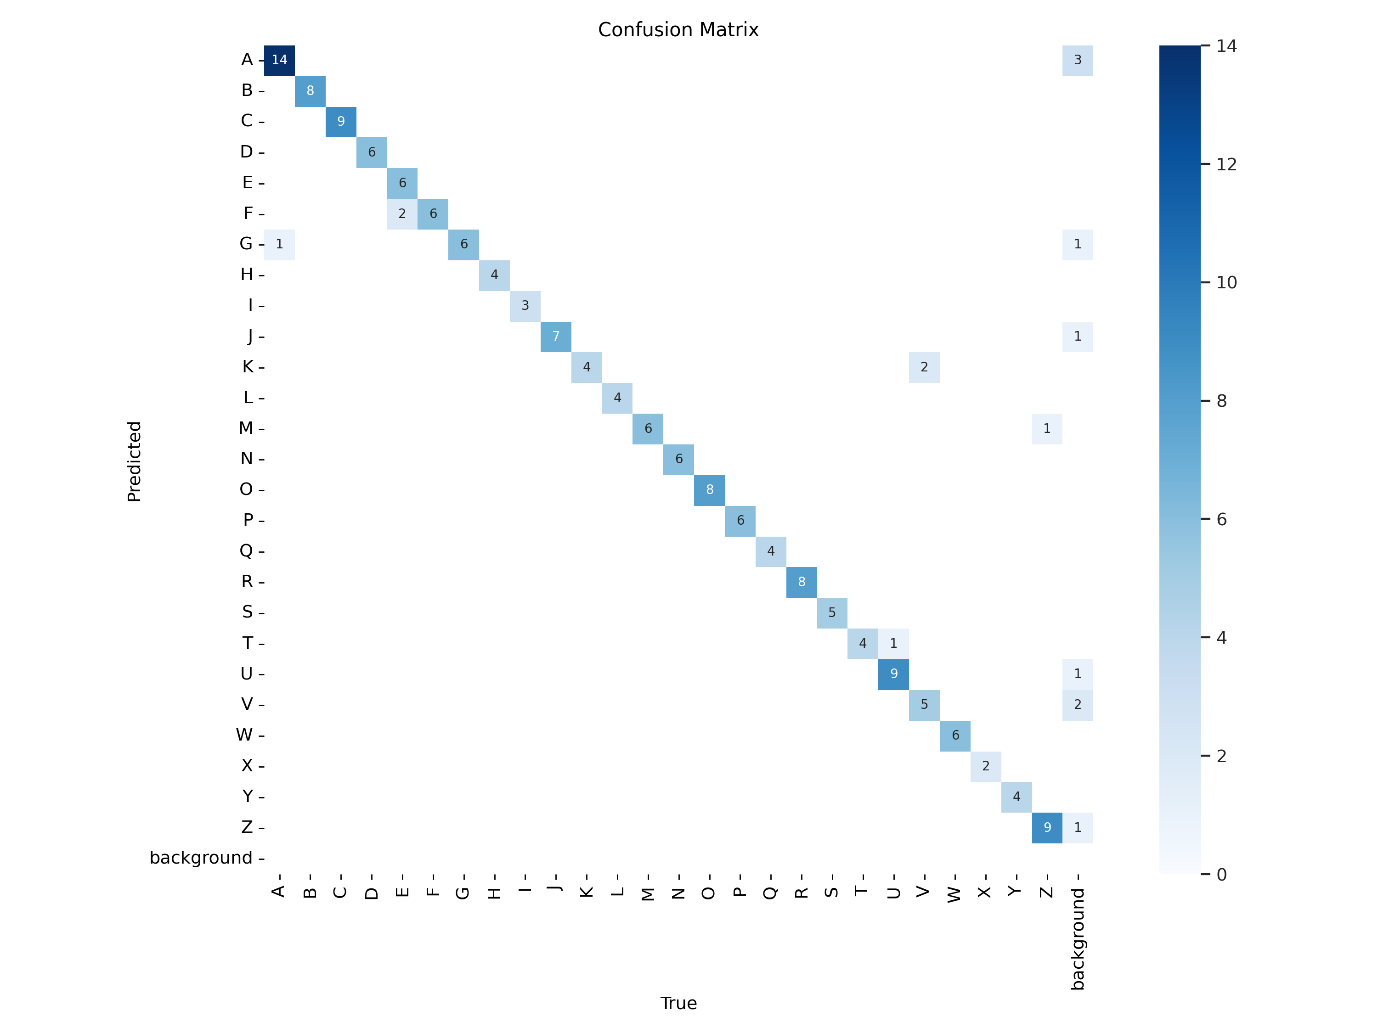
\includegraphics[width=0.6\linewidth]{Images/Gambar6Matrix.png}
    \caption*{Gambar 6. Confusion Matrix Model YOLOv5s}
    \label{fig:enter-label}
\end{figure}
\begin{adjustwidth}{6em}{0pt}
\hspace{0.5cm} Berdasarkan confusion matrix dari model YOLOv5s di atas, terlihat bahwa model telah mampu mengklasifikasikan sebagian besar kelas dengan cukup baik. Model ini mencakup 26 kelas utama (A hingga Z) serta kelas tambahan background yang berfungsi untuk menangani data yang tidak termasuk dalam kategori utama. Beberapa kelas seperti A, C, dan Z menunjukkan performa yang cukup baik, misalnya kelas A dengan 14 prediksi benar dan kelas Z dengan 9 prediksi benar. Namun, terdapat juga kesalahan klasifikasi yang signifikan, seperti sampel dari kelas F yang salah diklasifikasikan sebagai background sebanyak 2 kali, dan kelas background yang salah diprediksi ke kelas G sebanyak 1 kali. Kesalahan lain juga terlihat, misalnya pada kelas L yang salah diprediksi ke kelas lain sebanyak 2 kali. Hal ini menunjukkan bahwa meskipun model mampu menangani data dengan baik untuk sebagian besar kelas, masih terdapat tantangan dalam memisahkan kelas-kelas tertentu yang memiliki kemiripan fitur atau data dengan fitur yang tidak jelas. Penambahan kelas background membantu mengurangi noise dalam prediksi kelas utama, namun beberapa kesalahan prediksi ke kelas ini mengindikasikan bahwa model masih membutuhkan penyempurnaan, terutama pada data yang sulit diidentifikasi. Secara keseluruhan, performa model YOLOv5s cukup menjanjikan dengan potensi untuk peningkatan lebih lanjut, terutama dalam menangani kesalahan antar kelas.
\end{adjustwidth}

\begin{figure}[h]
    \centering
    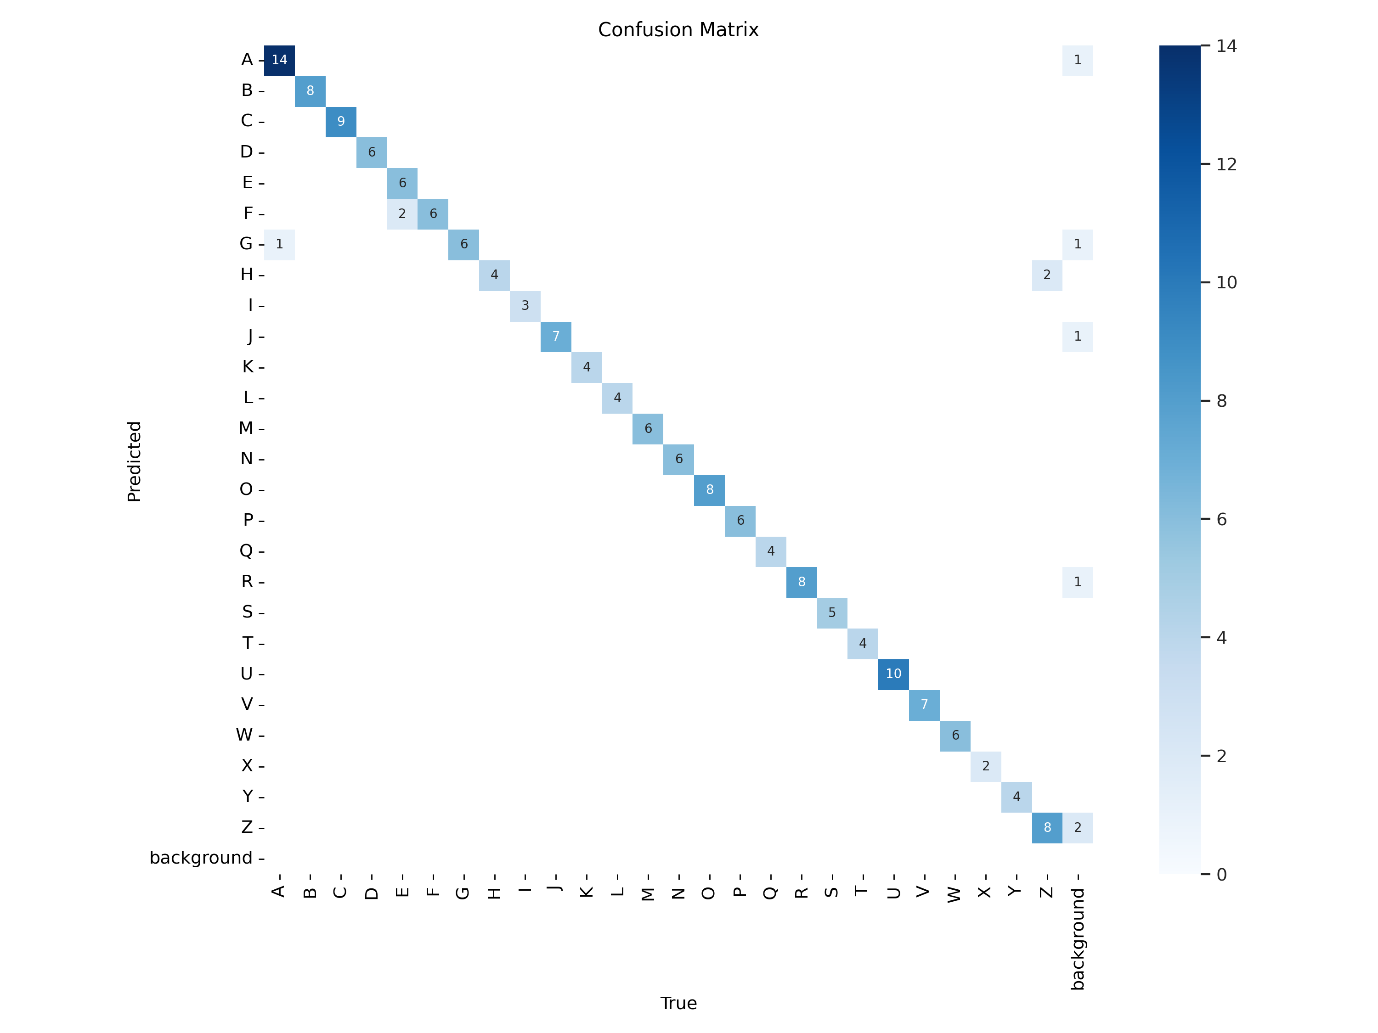
\includegraphics[width=0.6\linewidth]{Images/Gambar7Matrix.png}
    \caption*{Gambar 7. Confusion Matrix Model YOLOv8x}
    \label{fig:enter-label}
\end{figure}
\begin{adjustwidth}{3em}{0pt}
\hspace{0.5cm} Sementara confusion matrix dari model YOLOv8x di atas, terlihat bahwa model telah mampu mengklasifikasikan sebagian besar kelas dengan cukup baik. Model ini mencakup 26 kelas utama (A hingga Z) serta kelas tambahan background yang berfungsi untuk menangani data yang tidak termasuk dalam kategori utama. Beberapa kelas seperti A, C, dan U memiliki performa yang cukup tinggi, misalnya kelas A dengan 14 prediksi benar dan kelas U dengan 10 prediksi benar. Namun, terdapat juga kesalahan klasifikasi yang signifikan, seperti sampel dari kelas F yang salah diklasifikasikan sebagai background sebanyak 2 kali, dan kelas background yang salah diprediksi ke kelas G sebanyak 1 kali. Hal ini menunjukkan bahwa meskipun model mampu menangani data dengan baik untuk sebagian besar kelas, masih ada tantangan dalam memisahkan kelas yang saling mirip atau data dengan fitur yang kurang jelas. Penambahan kelas background membantu mengurangi noise dalam kelas utama, tetapi beberapa kesalahan prediksi ke kelas ini menunjukkan model masih membutuhkan penyempurnaan, terutama pada data yang sulit diidentifikasi. Secara keseluruhan, performa model YOLOv8x cukup menjanjikan dengan ruang untuk peningkatan, khususnya dalam menangani kesalahan antar kelas.
\end{adjustwidth}

\subsection{Visualization of Results}
\begin{adjustwidth}{3em}{0pt}
\hspace{0.5cm} Dalam percobaan ini, dua model yang berbeda dievaluasi untuk membandingkan kinerja mereka, yaitu YOLOv5s dan YOLOv8x. Kedua model tersebut dilatih untuk mendeteksi objek dengan metrik evaluasi yang meliputi precision, recall, dan mean average precision (mAP).
\begin{figure}[h]
    \centering
    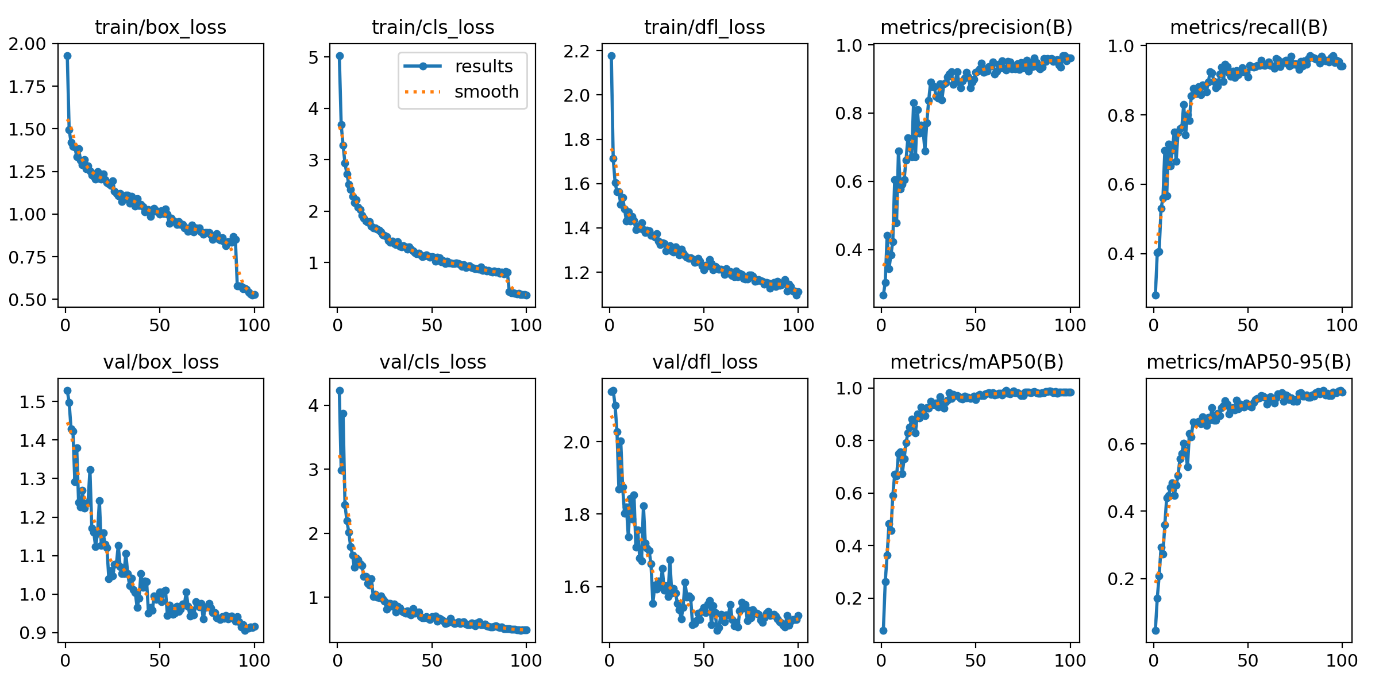
\includegraphics[width=0.6\linewidth]{Images/Gambar8Hasil.png}
    \caption*{Gambar 8. Hasil Dari Model YOLOv5s}
    \label{fig:enter-label}
\end{figure}


Model YOLOv5s menunjukkan kinerja yang cukup baik dengan tren penurunan nilai loss (box loss, classification loss, dan DFL loss) secara konsisten. Pada data validasi, precision dan recall model ini meningkat secara signifikan selama pelatihan, meskipun terdapat fluktuasi pada awal iterasi. Berikut adalah pengamatan utama dari model YOLOv5s:
\begin{itemize}
    \item Precision model meningkat stabil, mengindikasikan kemampuan model untuk menghindari kesalahan dalam mengklasifikasikan objek ke kelas yang salah.
    \item Recall juga meningkat dengan stabilitas yang lebih baik pada iterasi akhir, menunjukkan kemampuan yang memadai dalam mendeteksi objek-objek yang relevan.
    \item mAP@50 dan mAP@[50:95] menunjukkan peningkatan yang signifikan, menandakan kemampuan model untuk mendeteksi objek pada berbagai tingkat kesulitan dan IoU.

Secara keseluruhan, YOLOv5s bekerja dengan baik dalam menjaga keseimbangan antara precision dan recall, menghasilkan model yang andal meskipun sederhana
\end{itemize}
\begin{adjustwidth}{3em}{0pt}
\begin{figure}[h]
    \centering
    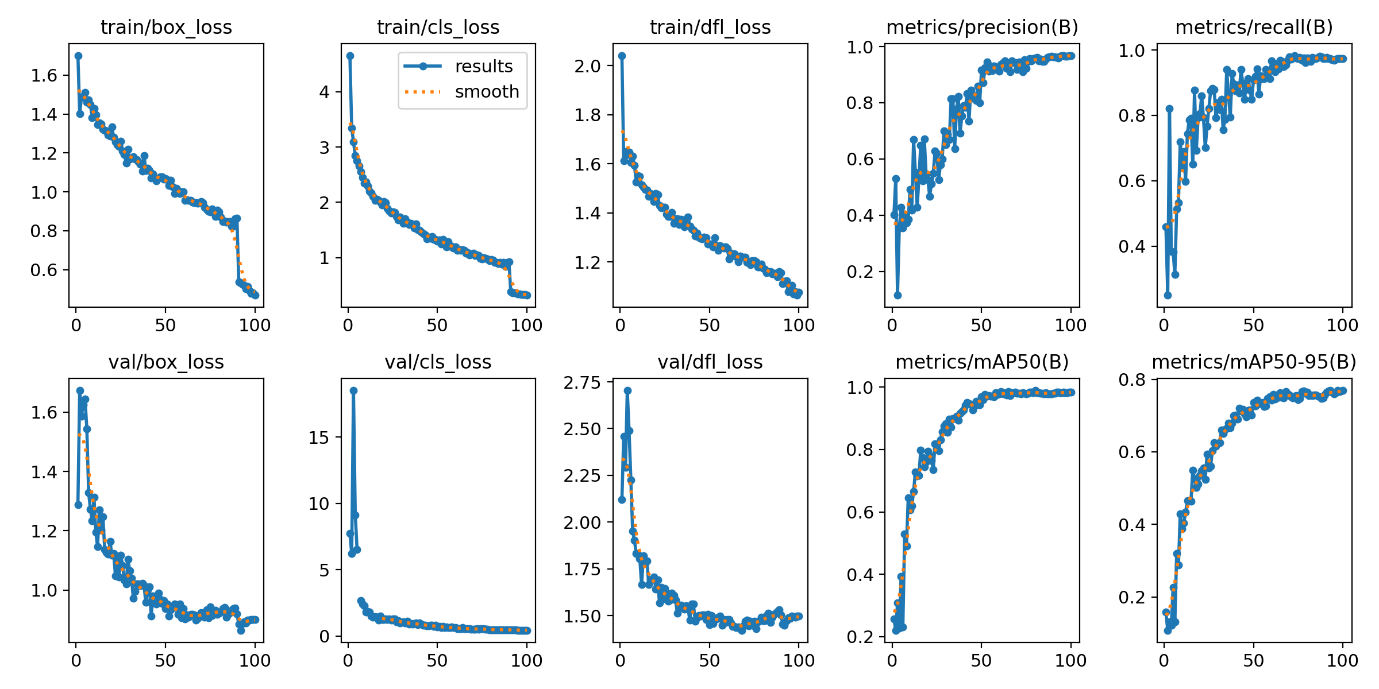
\includegraphics[width=0.6\linewidth]{Images/Gambar9Hasil.png}
    \caption*{Gambar 9. Hasil Dari Model YOLOv8x}
    \label{fig:enter-label}
\end{figure}
\hspace{0.5cm} 
\end{adjustwidth}

\hspace{0.5cm} Di sisi lain, model kedua, yaitu Model YOLOv8x, yang menggunakan arsitektur yang lebih kompleks dan modern, menunjukkan performa yang lebih unggul dibanding YOLOv5s. Hal ini terlihat dari penurunan nilai loss yang lebih cepat dan peningkatan stabil pada metrik evaluasi, seperti precision dan recall. Beberapa poin utama dari model YOLOv8x adalah sebagai berikut:
\begin{itemize}
    \item Precision model lebih tinggi dibanding YOLOv5s, menunjukkan bahwa model ini lebih berhati-hati dalam melakukan klasifikasi objek.
    \item Recall juga meningkat dengan stabilitas yang lebih baik, meskipun pada awal pelatihan terdapat fluktuasi kecil.
    \item mAP@50 dan mAP@[50:95] dari YOLOv8x lebih baik dibanding YOLOv5s, menunjukkan kemampuan deteksi objek yang lebih baik pada berbagai tingkat IoU.

Kinerja superior YOLOv8x ini menunjukkan bahwa model ini lebih mampu dalam mendeteksi objek secara akurat, mengurangi kesalahan klasifikasi, dan meningkatkan kemampuan generalisasi.
\end{itemize}
Secara keseluruhan, YOLOv8x terbukti menjadi model yang lebih unggul dibandingkan YOLOv5s. Meskipun YOLOv5s menunjukkan kinerja yang cukup baik dengan tren peningkatan pada precision, recall, dan mAP, model ini memiliki keterbatasan dibandingkan dengan YOLOv8x, terutama dalam hal kecepatan konvergensi dan stabilitas metrik evaluasi. YOLOv8x, dengan arsitektur yang lebih kompleks dan modern, tidak hanya menghasilkan precision dan recall yang lebih tinggi, tetapi juga memiliki mAP@50 dan mAP@[50:95] yang lebih baik, menunjukkan kemampuan yang lebih baik dalam mendeteksi objek pada berbagai tingkat kesulitan. Dengan penurunan nilai loss yang lebih cepat dan stabilitas metrik evaluasi yang lebih konsisten, YOLOv8x lebih andal dalam mendeteksi objek secara akurat, mengurangi kesalahan klasifikasi, dan meningkatkan kemampuan generalisasi. Oleh karena itu, YOLOv8x adalah pilihan yang lebih baik untuk tugas deteksi objek yang memerlukan kinerja tinggi dan presisi yang lebih akurat.
\end{adjustwidth}

\subsection{Discussion of the Results}
\begin{adjustwidth}{3em}{0pt}
\hspace{0.5cm} Hasil eksperimen ini menunjukkan adanya perbedaan performa signifikan antara model YOLOv5s dan YOLOv8x dalam mendeteksi gerakan bendera semaphore berdasarkan dataset yang telah dibuat. Beberapa poin penting yang dapat didiskusikan terkait hasil ini adalah:
\begin{itemize}
    \item Pengaruh Kompleksitas Model terhadap Precision dan Recall: Pada model YOLOv8x, precision cenderung lebih tinggi dibandingkan YOLOv5s. Hal ini disebabkan oleh arsitektur YOLOv8x yang lebih kompleks dan optimal untuk menangani variasi posisi tangan dan bendera yang lebih ambigu. Precision yang lebih tinggi pada YOLOv8x menunjukkan bahwa model ini lebih sedikit melakukan kesalahan klasifikasi ke kelas yang salah. Namun, seperti penelitian oleh Tobias Nagata Budimartono et al., kompleksitas tambahan sering kali membutuhkan sumber daya komputasi yang lebih besar. Di sisi lain, model YOLOv5s menunjukkan recall yang lebih tinggi, terutama pada gerakan-gerakan yang sederhana. Ini berarti model ini lebih sensitif dalam mendeteksi berbagai gerakan bendera, meskipun ada kemungkinan lebih besar untuk salah mengklasifikasikan gerakan ambigu. Hal ini serupa dengan temuan dari Athul Motty et al., yang menunjukkan bahwa model sederhana lebih responsif tetapi lebih rentan terhadap false positives.

    \item Kesamaan dengan Penelitian Sebelumnya: Penelitian Andhika Bayu Pangestu et al. menunjukkan bahwa algoritma YOLOv8 efektif dalam mendeteksi gerakan tangan pada Bahasa Isyarat Indonesia (BISINDO). Dalam eksperimen ini, YOLOv8x menunjukkan performa serupa, terutama dalam mengenali gerakan bendera yang memiliki fitur yang kompleks. Sebaliknya, model YOLOv5s lebih sesuai untuk pengenalan gerakan sederhana, seperti dalam penelitian Tobias N. Budimartono yang menggunakan sensor IMU.

    \item Tantangan dalam Deteksi Gerakan Semaphore: Salah satu tantangan utama dalam deteksi gerakan semaphore adalah variabilitas posisi tangan dan sudut bendera. Seperti yang diungkapkan dalam penelitian Hizkia Halim, keberhasilan deteksi seringkali dipengaruhi oleh keberagaman data pelatihan. Dalam eksperimen ini, model yang dilatih dengan dataset yang lebih kaya pada variasi sudut (dengan kategori tambahan untuk posisi tidak valid) cenderung memiliki precision lebih tinggi karena dapat memfilter noise lebih baik. Namun, recall model menurun karena beberapa gerakan yang sebenarnya valid terkategorikan sebagai "kelas lainnya." Hal ini konsisten dengan penelitian Batuhan Gündoğdu yang menekankan pentingnya preprocessing untuk meningkatkan akurasi pada dataset semaphore.

    \item Pengaruh Dataset terhadap Generalisasi Model: Penggunaan dataset semaphore dengan label sudut yang spesifik menunjukkan bahwa model mampu menggeneralisasi dengan baik pada variasi data pelatihan. Penelitian Tobias N. Budimartono et al. dan Batuhan Gündoğdu menunjukkan bahwa dataset dengan fitur yang representatif sangat penting untuk memastikan model dapat mengenali gerakan semaphore dalam kondisi yang berbeda. Dalam eksperimen ini, YOLOv8x menunjukkan keunggulan pada generalisasi data, tetapi membutuhkan waktu komputasi yang lebih lama. YOLOv5s, dengan arsitektur yang lebih ringan, menunjukkan performa lebih cepat namun kurang akurat pada kondisi data yang lebih kompleks..

    \item Kompleksitas dan Trade-Off Precision-Recall:Model YOLOv5s cenderung memiliki recall lebih tinggi tetapi precision lebih rendah karena fokusnya pada deteksi semua kemungkinan gerakan, termasuk yang ambigu. Sebaliknya, YOLOv8x lebih selektif, yang menghasilkan precision tinggi tetapi recall yang sedikit lebih rendah. Seperti yang disebutkan oleh penelitian Athul Motty et al., trade-off antara precision dan recall ini sangat penting untuk diaplikasikan sesuai kebutuhan, terutama dalam sistem real-time. 
    \end{itemize}

\hspace{0.5cm} Secara keseluruhan, eksperimen ini menunjukkan bahwa kompleksitas model dan pengaruh dataset memainkan peran penting dalam performa deteksi gerakan bendera semaphore. Model YOLOv8x, dengan arsitektur yang lebih kompleks, berhasil mencapai precision yang lebih tinggi dengan mengurangi kesalahan klasifikasi, terutama pada gerakan-gerakan dengan fitur yang lebih kompleks. Namun, peningkatan kompleksitas ini disertai dengan sedikit penurunan recall, karena model lebih selektif dalam deteksinya. Sebaliknya, YOLOv5s, dengan arsitektur yang lebih sederhana, menunjukkan recall yang lebih tinggi pada gerakan sederhana, tetapi precision-nya lebih rendah karena model lebih rentan terhadap false positives. Penggunaan dataset yang kaya dengan variasi sudut dan posisi terbukti membantu meningkatkan generalisasi model, terutama pada YOLOv8x, meskipun membutuhkan sumber daya komputasi yang lebih besar. Secara keseluruhan, hasil ini konsisten dengan penelitian sebelumnya, menunjukkan bahwa ada trade-off antara precision dan recall yang harus disesuaikan dengan kebutuhan aplikasi. Untuk mencapai kinerja yang optimal, diperlukan penggunaan model deteksi yang lebih canggih atau pengayaan dataset yang lebih representatif sesuai dengan kondisi nyata.

\end{adjustwidth}

% 5. Conclusion
\section{CONCLUSION}
\begin{adjustwidth}{3em}{0pt}
\subsection{Rekap Tujuan dan Pencapaian}
\hspace{0.5cm} Proyek ini bertujuan untuk membuat sistem deteksi gerakan bendera semaphore berbasis komputer visi dengan menggunakan model deep learning, khususnya YOLOv8. Tujuan ini telah berhasil dicapai melalui langkah-langkah berikut:
\begin{itemize}
    \item Pengembangan dataset: Dataset berisi gambar-gambar gerakan bendera semaphore dari berbagai posisi tangan kanan dan kiri sesuai kode semaphore, mencakup semua huruf alfabet.
    \item Implementasi model YOLOv8: Model berhasil mendeteksi gerakan bendera semaphore dengan tingkat akurasi yang cukup baik pada kondisi standar.
\end{itemize}

\subsection{Wawasan Utama dari Hasil}
\begin{itemize}
    \item Efektivitas Model Deep Learning: Model YOLOv8 menunjukkan kemampuan deteksi yang memadai, terutama pada kondisi pencahayaan normal. Namun, performa model menurun pada pencahayaan rendah atau sudut kamera yang tidak sesuai.
    \item Pengaruh Faktor Lingkungan: Akurasi deteksi berkurang akibat faktor lingkungan, seperti pencahayaan redup, latar belakang yang kompleks, atau gerakan tangan yang tidak konsisten. Hal ini mengindikasikan perlunya augmentasi data dan algoritma yang lebih tangguh.
    \item Potensi untuk Real-Time Processing: Sistem deteksi ini memiliki potensi untuk digunakan secara real-time, misalnya pada aplikasi komunikasi visual berbasis semaphore.
    \item Kontribusi untuk Aplikasi Pembelajaran: Dataset dan model ini dapat menjadi alat pembelajaran penting dalam memahami dan mengaplikasikan gerakan semaphore, baik untuk pelatihan individu maupun institusi.
\end{itemize}

\subsection{Pekerjaan dan Rekomendasi di Masa Depan}
\begin{itemize}
    \item Pengembangan Dataset Lebih Lanjut: Perluasan dataset dengan menambahkan variasi kondisi, seperti pencahayaan malam, sudut kamera berbeda, atau posisi tangan yang lebih dinamis, untuk meningkatkan robusta model.
    \item Peningkatan Model Deep Learning: Fine-tuning YOLOv8 atau eksplorasi model baru seperti YOLOv11 dan metode berbasis Transformer untuk meningkatkan akurasi pada kondisi non-ideal.
    \item Integrasi dengan Sistem Pembelajaran dan Komunikasi: Mengembangkan aplikasi desktop atau mobile untuk deteksi semaphore secara real-time dengan integrasi antarmuka pengguna interaktif.
    \item Sistem Deteksi Berbasis Cloud: Implementasi sistem berbasis cloud yang memungkinkan pengguna berbagi informasi gerakan semaphore secara otomatis untuk komunikasi jarak jauh.
    \item Kolaborasi dengan Peneliti Lain: Bermitra dengan peneliti di bidang bahasa isyarat atau semaphore untuk meningkatkan akurasi model dan memperluas penerapannya.
\end{itemize}
\hspace{0.5cm} Proyek ini merupakan langkah awal yang signifikan dalam memanfaatkan teknologi visi komputer untuk mendeteksi dan memahami gerakan semaphore. Hasilnya dapat digunakan untuk mendukung aplikasi komunikasi alternatif, pelatihan, dan pendidikan berbasis teknologi di berbagai bidang.

\end{adjustwidth}
\newpage
\begin{thebibliography}{99}
\begin{enumerate}
    \item Pangestu, A.B.; Muttaqin, M.R.; Sunandar, M.A. Sistem Deteksi Bahasa Isyarat Indonesia (BISINDO) Menggunakan Algoritma You Only Look Once (YOLO)v8. Teknik Informatika, STT Wastukancana Purwakarta. Jalan Cikopak No.53, Mulyamekar, Kec. Babakancikao, Kab. Purwakarta, Jawa Barat, Indonesia. \textbf{2024},   
    Available online: \url{https://www.ejournal.itn.ac.id/index.php/jati/article/view/10833/6205} (accessed on 2024).

    \item Halim, H.; Lina. Aplikasi Pengidentifikasi Bahasa Isyarat Berdasarkan Gerak Tubuh Secara Real Time Menggunakan YOLO. Fakultas Teknologi Informasi, Universitas Tarumanagara. \textbf{2023},
    Available online: \url{https://ejournal.catursakti.ac.id/index.php/simtek/article/view/215/230 } (accessed on 2023).
    
    \item Amri, I. Implementasi Algoritma Convolutional Neural Network untuk Menerjemahkan Bahasa Isyarat. \textbf{2024}, 
    Available online: \url{https://ejournal.warunayama.org/index.php/kohesi/article/view/2577/2427} (accessed on 2024).
    
    \item Motty, A.; Yogitha, A.; Nandakumar, R. Flag Semaphore Detection Using TensorFlow and OpenCV. \textbf{2019}.  
    Available online: \url{https://www.ijrte.org/wp-content/uploads/papers/v7i6/F2472037619.pdf} (accessed on 2019).
    
    \item Budimartono, T.N.; Widodo, R.B.; Irawan, P.L.T. Perancangan Aplikasi Realtime Berbasis Desktop dengan Sensor IMU pada Klasifikasi Gerakan Semaphore Menggunakan Metode CNN. Pusat Studi Human-Machine Interaction, Teknik Informatika, Universitas Ma Chung. Jalan Villa Puncak Tidar Blok N-1, Malang, Indonesia, 65151.\textbf{2022}.  
    Available online: \url{https://ocs.machung.ac.id/index.php/seminarnasionalmachung/article/view/328/176} (accessed on 2022).
    
    \item Budimartono, T.N.; Widodo, R.B. Studi Klasifikasi Gerakan Semaphore Menggunakan Fuzzy Mamdani dari Data IMU Sensor. \textbf{2023}.  
    Available online: \url{https://jurnal.istts.ac.id/index.php/INSYST/article/view/263/158} (accessed on 2023).
    
    \item Gündoğdu, B.; Kumlu, D. Clustering-Based Feature Extraction Methods for Semaphore Flag Recognition. \textbf{2020}.  
    Available online: \url{https://www.researchgate.net/publication/345719149_CLUSTERING_BASED_FEATURE_EXTRACTION_METHODS_FOR_SEMAPHORE_FLAG_RECOGNITION} (accessed on 2020).
    
\end{enumerate}
\end{thebibliography}
\end{document}